% 2011 浙江卷(理) 第21题 图: 抛物线、圆C2与过P的两条切线及直线l
\usetikzlibrary{arrows.meta,calc}
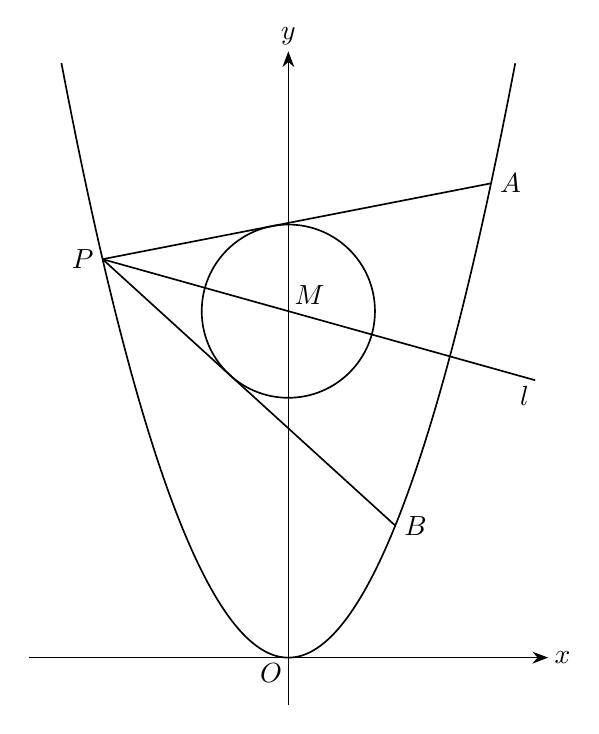
\begin{tikzpicture}[x=1cm,y=1cm,line width=.6pt,font=\normalsize,>=Stealth]
%==DATA-START== do not reorder
\def\scale{1.1}
\def\rC{1.1}
\def\xmax{2.882}
\coordinate (O) at (0.0,0.0);
\coordinate (M) at (0.0,4.4);
\coordinate (P) at (-2.359237164847994,5.06);
\coordinate (A) at (2.5740788489384863,6.023529018684074);
\coordinate (B) at (1.357983092474838,1.676470981315931);
\coordinate (Lend) at (3.135,3.5229792278499854);
\coordinate (Xone) at (-3.3,0.0);
\coordinate (Xtwo) at (3.3,0.0);
\coordinate (Yone) at (0.0,-0.605);
\coordinate (Ytwo) at (0.0,7.7);
%==DATA-END==
\draw[->] (Xone)--(Xtwo) node[right=2pt,inner sep=0pt] {$x$};
\draw[->] (Yone)--(Ytwo) node[above=2pt,inner sep=0pt] {$y$};
\draw[domain=-\xmax:\xmax,samples=141,smooth] plot (\x,{(\x)*(\x)/\scale});
\draw (M) circle [radius=\rC cm];
\draw (P)--(A);
\draw (P)--(B);
\draw (P)--(Lend);
\node[below left,inner sep=0pt,xshift=-2pt,yshift=-2pt] at (O) {$O$};
\node[above right,inner sep=0pt,xshift=2pt,yshift=2pt] at (M) {$M$};
\node[left,inner sep=0pt,xshift=-3pt] at (P) {$P$};
\node[right,inner sep=0pt,xshift=3pt] at (A) {$A$};
\node[right,inner sep=0pt,xshift=3pt] at (B) {$B$};
\node[below left,inner sep=0pt,xshift=-2pt,yshift=-2pt] at (Lend) {$l$};
\end{tikzpicture}
